\subsubsection{Caso d'uso UC8.1.7: Creazione domanda a ordinamento di stringhe}
	\label{UC8.1.7}
	\begin{figure}[ht]
		\centering
			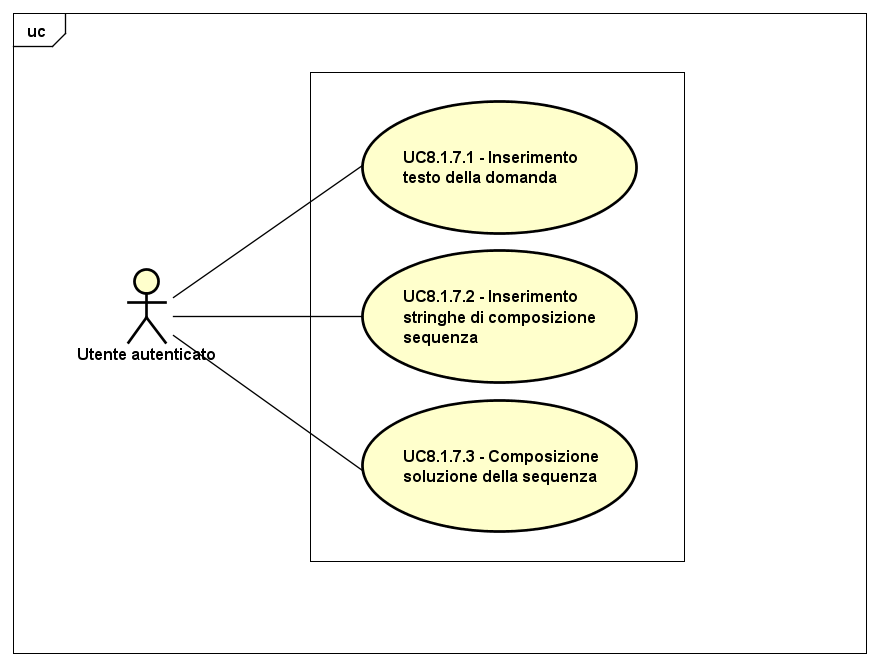
\includegraphics[scale=0.45,keepaspectratio]{UML/UC8_1_7.png}
		\caption{UC8.1.7: Creazione domanda a ordinamento di stringhe}
	\end{figure}
	\FloatBarrier
\begin{itemize}
	\item\textbf{Attori}: utente autenticato, utente autenticato pro;
	\item\textbf{Descrizione}: l'attore può utilizzare la procedura guidata per la creazione di una domanda a ordinamento di stringhe;
	\item \textbf{Precondizione}: il sistema presenta all'attore la procedura guidata per la creazione di una domanda a ordinamento di stringhe; 
	\item\textbf{Postcondizione}: l'attore ha creato una domanda a ordinamento di stringhe;
	\item\textbf{Scenario principale}:
		\begin{enumerate}
			\item L'attore può inserire il testo della domanda (UC8.1.7.1);
			\item L'attore può inserire le stringhe che compongono la risposta (UC8.1.7.2);
			\item L'attore può indicare la soluzione della sequenza di stringhe (UC8.1.7.3).
		\end{enumerate}
\end{itemize}

\subsubsection{Caso d'uso UC8.1.7.1: Inserimento testo della domanda}
	\begin{itemize}
		\item \textbf{Attori}: utente autenticato, utente autenticato pro;
		\item \textbf{Descrizione}: l'attore può inserire il testo della domanda;
		\item\textbf{Precondizione}: il sistema presenta all'attore lo spazio destinato all'inserimento del testo della domanda;
		\item \textbf{Postcondizione}: l'attore ha inserito il testo della domanda;
		\item\textbf{Scenario principale}: l'attore inserisce il testo della domanda.
	\end{itemize}
	
\subsubsection{Caso d'uso UC8.1.7.2: Inserimento stringhe di composizione sequenza}
	\begin{itemize}
		\item \textbf{Attori}: utente autenticato, utente autenticato pro;
		\item \textbf{Descrizione}: l'attore può inserire le stringhe che costituiscono la risposta alla domanda;
		\item\textbf{Precondizione}: il sistema presenta all'attore la funzionalità di inserire le stringhe che costituiscono la risposta alla domanda;
		\item \textbf{Postcondizione}: l'attore ha inserito le stringhe che costituiscono la risposta alla domanda;
		\item\textbf{Scenario principale}: l'attore inserisce le stringhe che costituiscono la risposta alla domanda.
	\end{itemize}
	
\subsubsection{Caso d'uso UC8.1.7.3: Composizione soluzione della sequenza}
	\begin{itemize}
		\item \textbf{Attori}: utente autenticato, utente autenticato pro;
		\item \textbf{Descrizione}: l'attore può indicare la soluzione della domanda mettendo nell'ordine corretto la sequenza di stringhe;
		\item\textbf{Precondizione}: il sistema presenta all'attore la funzionalità di indicare la soluzione della sequenza;
		\item \textbf{Postcondizione}: l'attore ha indicato la soluzione della sequenza;
		\item\textbf{Scenario principale}: l'attore indica la soluzione della sequenza. 
	\end{itemize}
